% ============================================================
%  RESTRUCTURED 2026-08-16. Survey-only chapter:
%  - "RAG Challenges and Solutions" moved to ProblemAndChallenges.tex
%    (challenges are part of the problem statement, not the survey).
%  - Bold-paragraph headers promoted to real sections.
%  - New TODO subsection for post-2025 developments.
%  All original prose kept verbatim; TODOs mark where to extend.
% ============================================================

\chapter{State of the Art} \label{ch:sota}

Recent advancements in Natural Language Processing (NLP) have seen the emergence of Retrieval-Augmented Generation (RAG) models, which combine the strengths of retrieval-based and generative approaches \cite{rag-nlp}. RAG has demonstrated significant potential in tasks requiring domain-specific knowledge and up-to-date information, addressing key limitations of traditional Large Language Models (LLMs), such as their tendency to generate inaccurate or irrelevant outputs. However, despite its growing adoption in various domains, the application of RAG to political texts—particularly in low-resource languages like Portuguese—remains underexplored.

\TODO{Tense/framing pass: this chapter was written in early 2025 for the
pre-thesis. Update the framing to reflect that the survey informed choices you
went on to make.}

\section{The RAG framework} \label{sec:sota-rag}

Retrieval-Augmented Generation (RAG) is a hybrid framework that enhances the capabilities of LLMs by integrating external data retrieval into the text generation process. Unlike traditional LLMs, which rely solely on pre-trained knowledge, RAG dynamically retrieves relevant document chunks from an external knowledge base using techniques such as dense vector retrieval and semantic similarity. This retrieval mechanism ensures that the generated outputs are grounded in factual and contextually appropriate information, significantly reducing the risk of hallucinations or inaccuracies commonly associated with standalone LLMs \cite{rag-nlp, zhang2023sirenssongaiocean}. By combining the generative power of LLMs with the ability to access and incorporate external knowledge, RAG represents a significant advancement in knowledge-intensive NLP tasks.

\subsection{The RAG pipeline} \label{subsec:sota-pipeline}

A RAG pipeline consists of several key components, each playing a critical role in the retrieval and generation process. At its core, the pipeline integrates two main stages: \textbf{retrieval}, where relevant documents are fetched from an external knowledge base, and \textbf{generation}, where a language model synthesizes the retrieved information into a coherent response. See Figure \ref{fig:rag-diagram} for an overview of a simple RAG process.

\begin{figure}[h]
\begin{center}
    \copyrightbox{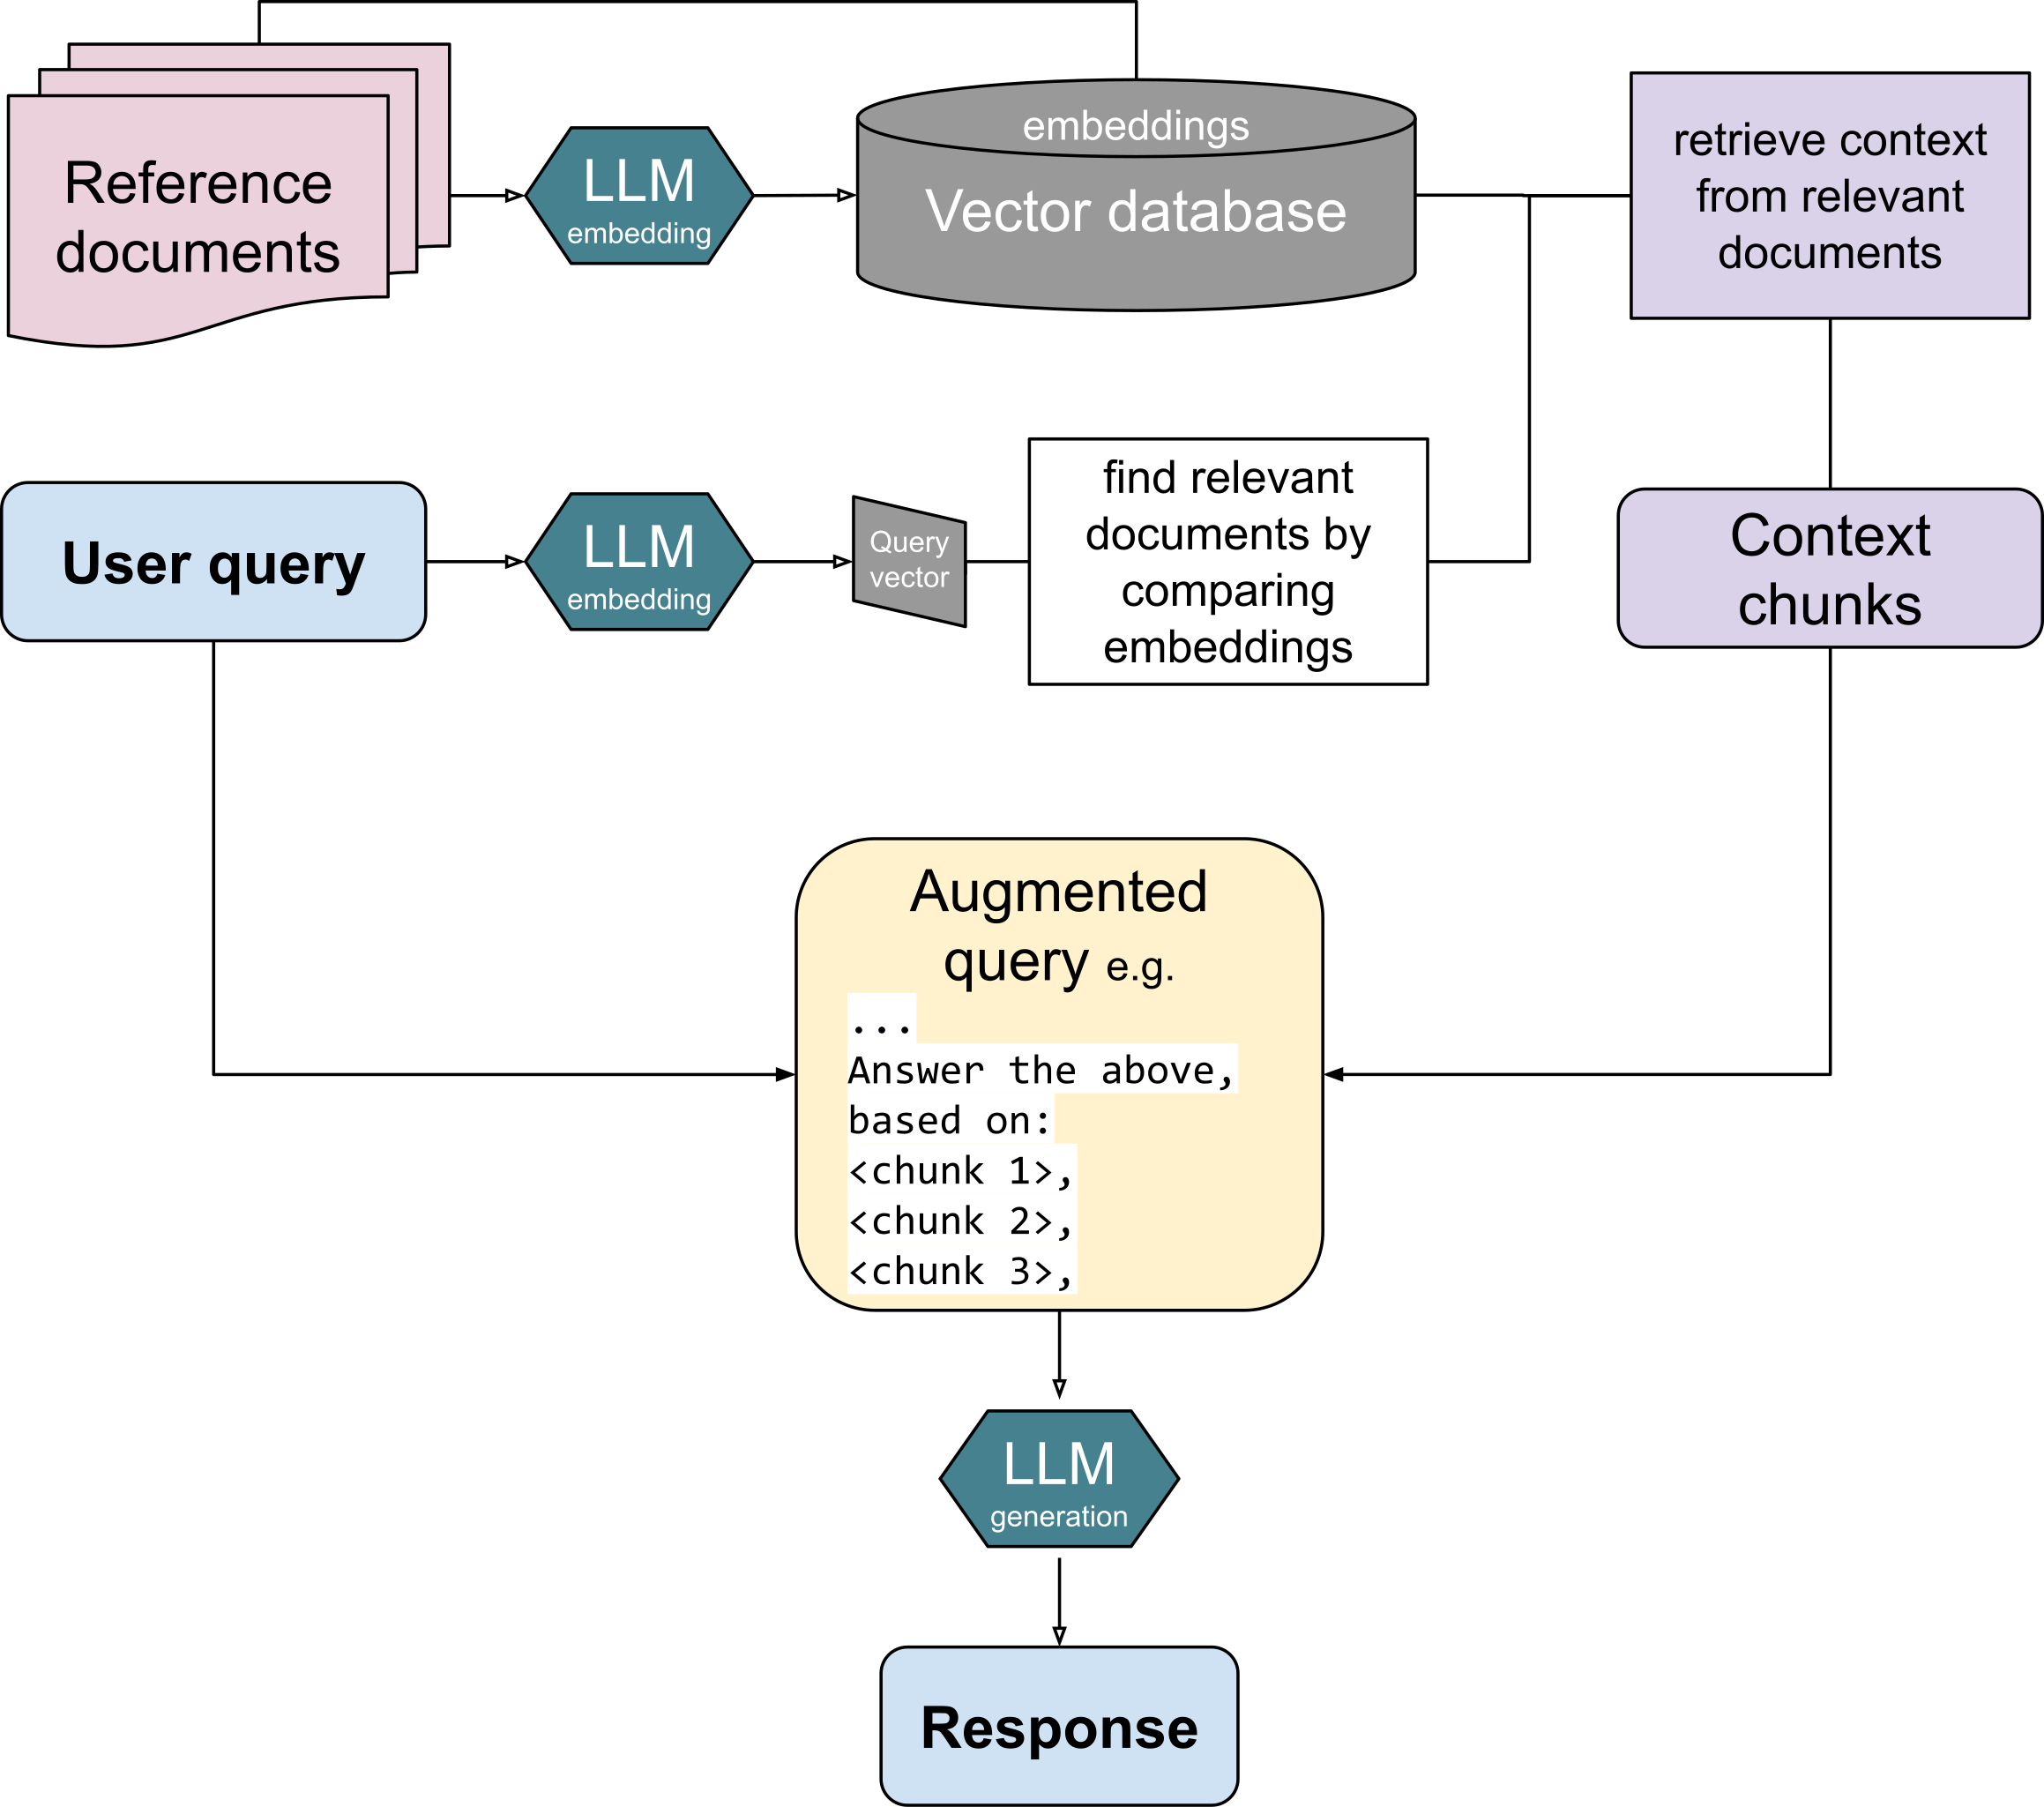
\includegraphics[width=0.8\textwidth]{images/RAG-diagram.png}}{By Turtlecrown - Own work, CC BY-SA 4.0,\\https://commons.wikimedia.org/w/index.php?curid=150390279}
\end{center}
\caption{Overview of a RAG process}
\label{fig:rag-diagram}
\end{figure}

\subsection{Advanced RAG variants} \label{subsec:sota-variants}

The Retrieval-Augmented Generation (RAG) framework, introduced by \cite{rag-nlp}, combines a pre-trained retriever with a sequence-to-sequence (seq2seq) model, fine-tuned end-to-end. This integration enables the model to generate accurate, contextually grounded responses by leveraging external knowledge.

Building on this, Self-RAG \cite{asai2024selfrag} introduces a self-reflective mechanism to dynamically assess retrieval and generation quality, improving efficiency and accuracy. Similarly, Corrective RAG (CRAG) \cite{crag} adds a lightweight retrieval evaluator to assess the overall quality of retrieved documents for a query, returning a confidence degree based on which different knowledge retrieval actions can be triggered. More recently, Agentic RAG \cite{agentic-rag} has emerged as an advanced paradigm by embedding autonomous AI agents into the RAG pipeline. These agents leverage agentic design patterns reflection, planning, tool use, and multiagent collaboration to dynamically manage retrieval strategies, iteratively refine contextual understanding, and adapt workflows to meet complex task requirements.

\subsection{Recent developments} \label{subsec:sota-recent}

\TODO{NEW subsection: the field moved fast during this work (a core thesis
theme). Survey what appeared after the pre-thesis (2025--2026): retrieval-tuned
embedding families (e.g.\ Qwen3-Embedding), reranker models, hybrid
dense+lexical retrieval as standard practice, RAG evaluation frameworks
(RAGAS-style, LLM-as-judge), and the technique series you drew from
(RAG-from-Scratch). This subsection justifies WHY choices were revisited
mid-project --- link it to the decision-history narrative in
Chapter~\ref{ch:proposition}.}

\subsection{Is retrieval still worth it?} \label{subsec:sota-why-rag}
%% DRAFT (Claude, 2026-10-10): to be read and rewritten in the author's own words.
\TODO{REVIEW: Claude's draft of this subsection (2026-10-10). Read it, trim
and sharpen it, and rewrite it in your own voice. The 750k-token corpus size
was measured with the Qwen3-Embedding tokenizer; other tokenizers will differ
somewhat.}

Every jump in context length revives the same obituary: why retrieve a few
passages when the model can simply read everything? The windows went from
thousands of tokens to a million, and ``RAG is dead'' became a recurring
industry refrain. For a corpus like this one, the obituary is premature.
Six reasons:

\begin{description}
    \item[Reading everything is not reading well.] Long-context models use
    their input unevenly. Information in the middle of a long prompt is used
    worse than information at its edges~\citep{liu2024lostinthemiddle}, and
    performance grows less reliable as the input grows, even on simple
    tasks~\citep{hong2025contextrot}. A shortlist of relevant passages gives
    the model less to get lost in.
    \item[Reading everything is expensive.] The eight manifestos come to
    roughly 750 thousand tokens. Sending them with every question means paying
    for the whole corpus every time; \sysname{} sends at most 16 thousand,
    about fifty times less. A controlled comparison found that long-context
    models outperform RAG on average when resources are unlimited, while RAG
    costs far less~\citep{li2024ragorlongcontext}. A civic tool meant to be
    free does not have unlimited resources.
    \item[The long tail is not in the weights.] Models remember popular facts
    well and rare ones badly~\citep{kandpal2023largelanguagemodelsstruggle}.
    A small party's housing proposal, written in European Portuguese, is about
    as long-tail as knowledge gets.
    \item[Receipts.] Every claim in a RAG answer can cite the passage it came
    from. For political information the citation is the product: a reader who
    doubts an answer can check it in seconds.
    \item[The parties' words, not the model's.] Language models absorb
    political leanings from their training
    data~\citep{pretraining-political-bias}. Grounding answers in the
    manifestos keeps the model reporting positions rather than holding them,
    and makes ``the manifestos do not say'' a legitimate answer instead of an
    invitation to improvise.
    \item[New election, same model.] Updating a RAG system means indexing new
    documents, not retraining a model. Adding a party outside parliament or a
    past election is a data task, and no answer depends on a training cutoff.
\end{description}

To be fair to the other side: retrieval brings failure modes of its own. A
passage that is never retrieved can never be cited, and
Chapter~\ref{ch:proposition} documents two failures that went unnoticed for
months. Hybrid designs such as Self-Route~\citep{li2024ragorlongcontext},
which answer from retrieved passages and fall back to the full context only
when those fall short, suggest the real answer is ``both, routed well''.
Whether \sysname{} earns its keep against a strong model with no retrieval at
all is not argued here but measured: it is RQ5
(Section~\ref{sec:research-questions}).

\TODO{Decide: keep or drop an embeddings survey subsection here. There is a
commented-out draft below; candidate-model detail may fit better in
Section~\ref{subsec:embeddings}. If kept here, survey encoder
FAMILIES and benchmarks (MTEB), not your specific candidates.}

\begin{comment}
\subsection{Embeddings}

% Tem de ser melhorado

Embeddings play a crucial role in the RAG pipeline, as they encode the semantic meaning of words, phrases, or documents into numerical representations that machines can process. By transforming text into dense vector spaces, embeddings enable tasks such as semantic similarity calculation, which is essential for retrieving relevant documents and generating contextually appropriate responses.
\end{comment}

\section{NLP for political text analysis} \label{sec:sota-political}

The analysis of political texts, such as electoral programs and manifestos, has been a growing area of interest in NLP. Studies have applied various techniques, including topic modeling, sentiment analysis, and semantic similarity, to analyze electoral programs in multiple languages \cite{manifestos-central-eastern, manifestos-nz}.

In the context of the Portuguese language, \cite{rag-chatbot} demonstrated the application of RAG in developing conversational agents, while \cite{paula-etal-2024-evaluation} applied two Question Answering Generation (QAG) approaches to generate question-answer pairs for three domains in Portuguese using different decoding methods. The recent work by \cite{marino-etal-2024-decoding} has explored the decoding of political discourse, highlighting the unique linguistic and cultural nuances of Portuguese electoral programs. However, these studies have primarily relied on traditional NLP methods or have focused on applying RAG to domains other than political text analysis.

\TODO{Expand related work: you have unused bib entries that belong here
(political-rag, givers-takers, llm-future, laver\_benoit\_garry is cited only
in the Introduction). Position your work against them: what does a
RAG-over-manifestos system do that manifesto-NLP classifiers and generic PT
chatbots do not?}

\section{Evaluate RAG systems} \label{sec:sota-evaluate}

Evaluate RAG systems is a critical step in the development of RAG systems. It involves assessing the performance of the RAG system in terms of various metrics, such as accuracy, precision, recall, and F1 score. It also involves assessing the quality of the retrieved documents and the generation of the response.

\subsection{Metrics} \label{subsec:sota-metrics}

The metrics used to evaluate RAG systems are:


\begin{comment}
\section{Index}

In this example, several keywords\index{keywords} will be used
which are important and deserve to appear in the Index\index{Index}.

Terms like generate\index{generate} and some\index{others} will also
show up. Terms in the index can also be nested \index{Index!nested}.

Cf. the \texttt{dissertation.bib} file to see some index definitions like \uminho{UMinho}.
\end{comment}
